%%%%%%%%%%%%%%%%%%%%%%%%
\chapter{Chasing systematics}
\label{resultsa}
%%%%%%%%%%%%%%%%%%%%%%%%
%say that you first did some tests with different wavelength ranges and that you saw weird things
    \section{Impact of Earth's atmosphere and the interstellar medium on the spectra}
    \begin{figure}[H]
        \centering
        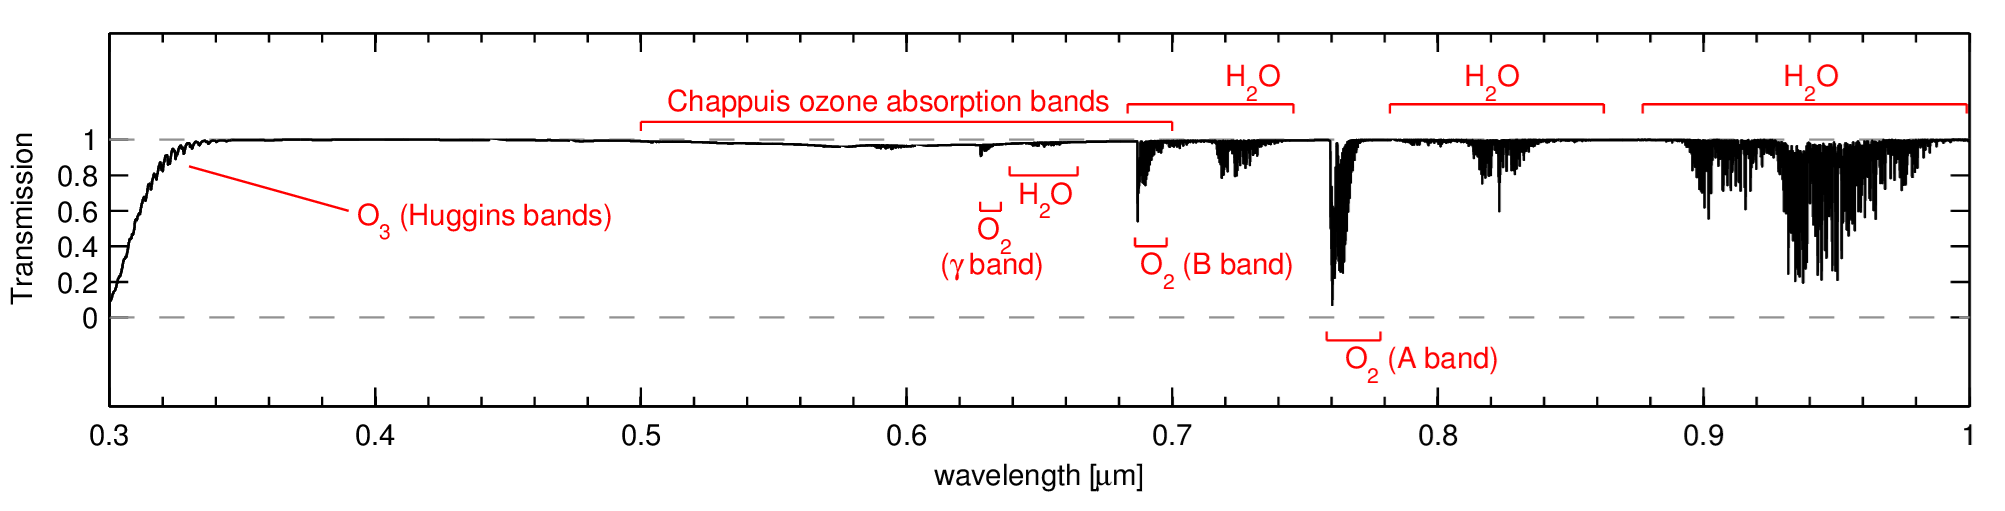
\includegraphics[width=\textwidth]{report/images/chap4_results/paranal_smette.png}
        \caption{Caption}
        \label{4.1a}
    \end{figure}
        \subsection{Tellurics}
        %test if by masking tellurics it works
        \subsection{The sodium doublet}
        \subsection{Low-frequency variations and the influence of the wavelength range's size}
        %show comparison of peak power for shape and shift for different sizes using rassine and explain that since rv computed with whole spectrum then the bigger the wavelength range the better the results: the shift is well suppressed(maybe take the ratio of significance between shape and shift to show that it diminishes ? ) -> explain why: rvs are computed using an "averaged" spectral line. So it is an averaged rv. So two things: 1. Using a bigger range means we represent the rv better so the shift is better suppressed. 2. Parts of the spectra represent better the rv in question but that depends ultimately on the star and its own characteristics so there is probably no better range. The best is to have the rv used for the periodogram computed with the same spectra used in the periodogram.
    \section{Upward and downward trends in the partial periodograms}
    %do the fits maybe ? Use polaris and some other less pronounced star as examples. Say that it was already present in SMus
    %this trend makes me wonder if even the bootstrap to compute the fap is relevant.
    %if the number of observations is sufficient, applying rassine corrects the residual trend and it's all good. So basically the trend is due to several factors.
    %%%%%%%%%%%%%%%%%%%%
    %Explain that the dinosaur shapes are maybe some oversampling of the peaks because we have very few observations.
\chapter{Analysis of 15 Cepheids}
\label{resultsb}
    \section{CORALIE07}
    \section{CORALIE14}
    \section{HERMES}



